\documentclass{beamer}

\setbeamertemplate{itemize item}[ball]

\usepackage{algpseudocode}
\usepackage{algorithm}
\usepackage{float}
\algdef{SE}[DOWHILE]{Do}{doWhile}{\algorithmicdo}[1]{\algorithmicwhile\ #1}

\usepackage{amsmath}
\usepackage{amssymb}
\usepackage{amsthm}
\usepackage{bm}
\usepackage{tikz}
\usetikzlibrary{bayesnet}

\usetheme{Madrid}


\title{Local PC Algorithm}
\author{Stephen Smith}
\institute[UCLA]{University of California, Los Angeles}



\begin{document}

\frame{\titlepage}

\frame{\tableofcontents}

\section{Introduction}


\begin{frame}
\frametitle{Graphs}

\begin{exampleblock}{Definition (Graph)}
A graph $G = (V,E)$ consists of a set of nodes $V = \{1,\ldots,p\}$ and a set of edges $E \subseteq V \times V$ with ordered pairs of distinct nodes.\\
\vspace{10pt}
An edge $(i,j) \in E$ is called directed if $(j,i) \notin E$, and we use the notation $i \rightarrow j$.
\end{exampleblock}

The set of nodes correspond to the components of a random vector $\mathbf{X} \in \mathbb{R}^p$ \\
\vspace{10pt}
The structure of a graph $G$ can be represented in an adjacency matrix $A = (a_{ij})_{p \times p}$ where
$$ a_{ij} = 
\begin{cases}
1 & \textrm{if $(i,j) \in E$} \\
0 & \textrm{otherwise}
\end{cases}
$$
 
\end{frame}

\begin{frame}
\frametitle{ Directed Acyclic Graphs  }
\begin{exampleblock}{ Definition (DAG) }
A Directed Acyclic Graph (DAG) is a graph $\mathcal{G}$ where all edges are directed and there are no cycles
\end{exampleblock}

\begin{itemize}
\item A \textit{v-structure} in a DAG $\mathcal{G}$ is an ordered triple of nodes $(i,j,k)$ such that $\mathcal{G}$ contains the directed edges $i \rightarrow k$ and $j \rightarrow k$, where $i$ and $j$ are not adjacent. We will denote such a structure by $i \rightarrow k \leftarrow j$.
\item Two DAGs are \textit{equivalent} if and only if they have the same skeleton and v-structures.
\end{itemize}

\end{frame}

\begin{frame}{Bayesian Network}
\begin{exampleblock}{Definition}
Random variables $X = (X_1,\ldots, X_p)$ are a Bayesian Network with respect to a DAG $\mathcal{G}$ if the joint probability density function $P$ can be written as
$$ p(x) = \prod_{v \in V} p(x_v \mid x_{pa(v)}) $$
where $pa(v) = \{ v' \in V :  v' \rightarrow v\}$.
\end{exampleblock}
\end{frame}

\begin{frame}
\frametitle{Example}
This is an example of a Bayesian Network with 8 nodes (taken from the bnlearn online repository).
\begin{figure}
  \centering
  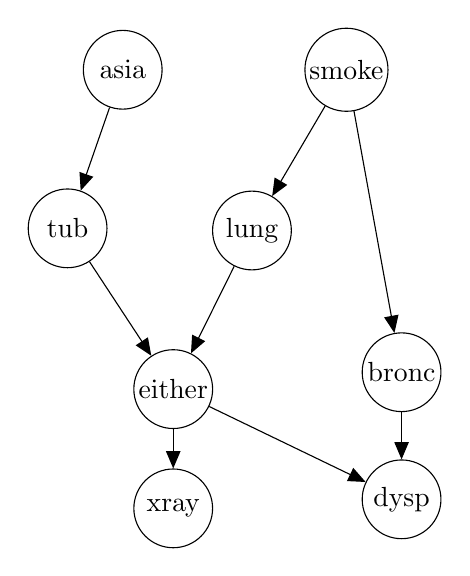
\begin{tikzpicture}[latent/.append style={minimum size=1cm},obs/.append style={minimum size=2cm}] %
    \node[latent] (asia) {asia} ; %
    \node[latent, right=of asia,xshift=0.8cm] (smoke) {smoke} ; %
    \node[latent, below=of asia,xshift=-0.7cm] (tub) {tub} ; %
    \node[latent, right=of tub, below=of smoke,xshift=-1.2cm] (lung) {lung};
    \node[latent, below=of lung,xshift=-1cm] (either) {either};
    \node[latent, below=of smoke,yshift=-1.8cm,xshift=0.7cm] (bronc) {bronc};
    \node[latent, below=of bronc,yshift=0.4cm] (dysp) {dysp};
    \node[latent, below=of either,yshift=0.5cm] (xray) {xray};
    \edge {asia}{tub} ; %
    \edge {tub}{either};
    \edge{lung}{either};
    \edge{smoke}{lung};
    \edge{smoke}{bronc};
    \edge{bronc}{dysp};
    \edge{either}{dysp};
    \edge{either}{xray};
  \end{tikzpicture}
\end{figure}

\end{frame}

\begin{frame}{Skeleton}

\begin{exampleblock}{ Definition (Skeleton) } 
The skeleton of a DAG $\mathcal{G}$ ignores the direction of the edges by substituting undirected edges for directed edges
\end{exampleblock}

A probability distribution $P$ on $\mathbb{R}^p$ is faithful with respect to a graph $G$ if conditional independence information of the distribution may be inferred from \textit{d-separation} in the graph $G$. 

\vspace{10pt}

The skeleton is highly interpretable and yields insights into the dependence structure of the data, thus it is valuable to estimate.

\end{frame}

\begin{frame}{PDAGs and CPDAGs}

\begin{exampleblock}{ PDAG }
A partially directed acyclic graph (PDAG) is a graph where some edges are directed and some are undirected, and no cycle may be traced following the directed edges and any direction for undirected edges.
\end{exampleblock}

\begin{exampleblock}{ CPDAG }
A CPDAG is a PDAG that is \textit{completed}, that is, it satisfies the following:
\begin{enumerate}
\item Every directed edge exists in every DAG belonging to the equivalence class of the DAG
\item For every undirected edge $i - j$, there exists a DAG with $i \rightarrow j$ and a DAG with $i \leftarrow j$ in the equivalence class.
\end{enumerate}
\end{exampleblock}
A CPDAG helps us to visualize \textit{equivalence classes}, and estimating this graph is the primary structure learning task of the PC algorithm.

\end{frame}





\section{Review of PC Algorithm}



\begin{frame}{PC Algorithm - Skeleton Estimation}


\begin{algorithm}[H]
\footnotesize
\caption{Population PC Algorithm}
\begin{algorithmic}[1]
\State \textbf{Input:} Vertex set $V$, Conditional Independence Information, $\ell_{max}$
\State Form the complete undirected graph $\tilde{C}$ on the vertex set $V$
\State $\ell = -1$; $C = \tilde{C}$
\While{$\ell < \ell_{max}$}
\State{$\ell = \ell + 1$}
\Do
\State Select a new, adjacent pair of ordered nodes $(i,j)$ s.t. $|adj(C,i) \setminus \{j\}| \geq \ell$
\Do
\State Choose new set $\mathbf{k} \subseteq adj(C,i)\setminus \{j\}$ with $|\mathbf{k}|=\ell$
\If{$i$ and $j$ are C.I. given $\mathbf{k}$}
\State Delete edge $i,j$; Save $\mathbf{k}$ in $S(i,j), S(j,i)$
\EndIf
\doWhile{$C_{ij}=1$ or there are new $\mathbf{k}$ to be chosen}
\doWhile{there remains ordered pairs with appropriately sized $\mathbf{k}$ to be tested for C.I.}
\EndWhile
\State \textbf{Output:} estimated skeleton $C$ and separation sets $S$
\end{algorithmic}
\end{algorithm}


\end{frame}


\begin{frame}{Population PC Algorithm - CPDAG Estimation}

Once we have the skeleton and the separation sets, we can orient some of the edges by finding v-structures and using Meek's rules.
\begin{algorithm}[H]
\footnotesize
\caption{V-Structure Orientation Algorithm}
\begin{algorithmic}[1]
\State \textbf{Input:} Skeleton $G$, Separation sets $S$
\For{pairs of nonadjacent $i,j$ with common neighbor $k$}
\If {$k \notin S(i,j)$}
\State Replace $i - k - j$ in $G$ with by $i \rightarrow k \leftarrow j$
\EndIf
\EndFor
\State Use Meek's Rules for edge orientation
\State \textbf{Output:} CPDAG $G$
\end{algorithmic}
\end{algorithm}


\end{frame}


\begin{frame}{Visual Demonstration of PC Algorithm}

\only<1>{
We start with a complete graph $\tilde{C}$
\begin{figure}
  \centering
  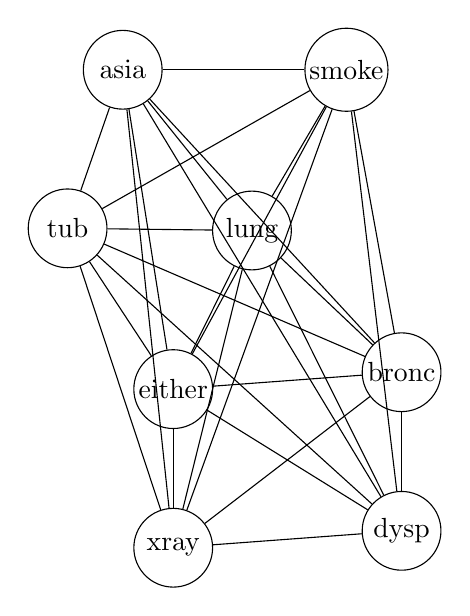
\begin{tikzpicture}[latent/.append style={minimum size=1cm},obs/.append style={minimum size=2cm}] %
    \node[latent] (asia) {asia} ; %
    \node[latent, right=of asia,xshift=0.8cm] (smoke) {smoke} ; %
    \node[latent, below=of asia,xshift=-0.7cm] (tub) {tub} ; %
    \node[latent, right=of tub, below=of smoke,xshift=-1.2cm] (lung) {lung};
    \node[latent, below=of lung,xshift=-1cm] (either) {either};
    \node[latent, below=of smoke,yshift=-1.8cm,xshift=0.7cm] (bronc) {bronc};
    \node[latent, below=of bronc] (dysp) {dysp};
    \node[latent, below=of either] (xray) {xray};
    \draw (asia)--(tub) ; %
    \draw (asia)--(xray) ;
    \draw (asia)--(either);
    \draw (asia)--(lung);
    \draw (asia)--(smoke);
    \draw (asia)--(dysp);
    \draw (asia)--(bronc);
    \draw (smoke)--(tub) ; %
    \draw (smoke)--(xray) ;
    \draw (smoke)--(either);
    \draw (smoke)--(lung);
    \draw (smoke)--(dysp);
    \draw (smoke)--(bronc);
    \draw (tub)--(xray) ;
    \draw (tub)--(either);
    \draw (tub)--(lung);
    \draw (tub)--(dysp);
    \draw (tub)--(bronc);
    \draw (xray)--(either);
    \draw (xray)--(lung);
    \draw (xray)--(dysp);
    \draw (xray)--(bronc);
    \draw (either)--(lung);
    \draw (either)--(dysp);
    \draw (either)--(bronc);
    \draw (lung)--(dysp);
    \draw (lung)--(bronc);
    \draw (dysp)--(bronc);
  \end{tikzpicture}
\end{figure}
}
\only<2>{
With $\ell=0$, we delete edges of $C$ that have insignificant correlations.
\begin{figure}
  \centering
  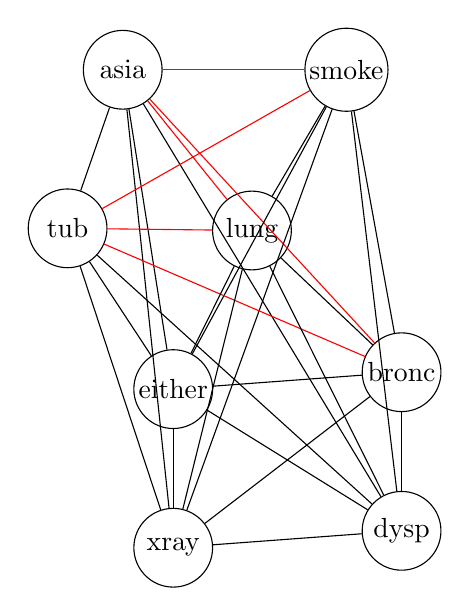
\begin{tikzpicture}[latent/.append style={minimum size=1cm},obs/.append style={minimum size=2cm}] %
    \node[latent] (asia) {asia} ; %
    \node[latent, right=of asia,xshift=0.8cm] (smoke) {smoke} ; %
    \node[latent, below=of asia,xshift=-0.7cm] (tub) {tub} ; %
    \node[latent, right=of tub, below=of smoke,xshift=-1.2cm] (lung) {lung};
    \node[latent, below=of lung,xshift=-1cm] (either) {either};
    \node[latent, below=of smoke,yshift=-1.8cm,xshift=0.7cm] (bronc) {bronc};
    \node[latent, below=of bronc] (dysp) {dysp};
    \node[latent, below=of either] (xray) {xray};
    \draw (asia)--(tub) ; %
    \draw (asia)--(xray) ;
    \draw (asia)--(either);
    \draw [red] (asia)--(lung);
    \draw [red] (asia)--(smoke);
    \draw (asia)--(dysp);
    \draw [red] (asia)--(bronc);
    \draw [red] (smoke)--(tub) ; %
    \draw (smoke)--(xray) ;
    \draw (smoke)--(either);
    \draw (smoke)--(lung);
    \draw (smoke)--(dysp);
    \draw (smoke)--(bronc);
    \draw  (tub)--(xray) ;
    \draw (tub)--(either);
    \draw [red] (tub)--(lung);
    \draw (tub)--(dysp);
    \draw [red] (tub)--(bronc);
    \draw (xray)--(either);
    \draw (xray)--(lung);
    \draw (xray)--(dysp);
    \draw (xray)--(bronc);
    \draw (either)--(lung);
    \draw (either)--(dysp);
    \draw (either)--(bronc);
    \draw (lung)--(dysp);
    \draw (lung)--(bronc);
    \draw (dysp)--(bronc);
  \end{tikzpicture}
\end{figure}
}
\only<3>{
With $\ell=1$, we delete edges $(i,j)$ with insignificant \textit{partial} correlations given a separation set $S_{ij}$.
\begin{figure}
  \centering
  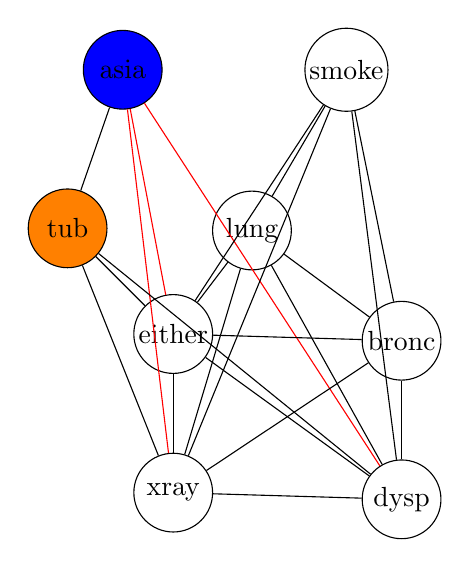
\begin{tikzpicture}[latent/.append style={minimum size=1cm},obs/.append style={minimum size=2cm}] %
    \node[latent, fill=blue] (asia) {asia} ; %
    \node[latent, right=of asia,xshift=0.8cm] (smoke) {smoke} ; %
    \node[latent, below=of asia,xshift=-0.7cm,fill=orange] (tub) {tub} ; %
    \node[latent, right=of tub, below=of smoke,xshift=-1.2cm] (lung) {lung};
    \node[latent, below=of lung,xshift=-1cm,yshift=0.7cm] (either) {either};
    \node[latent, below=of smoke,yshift=-1.4cm,xshift=0.7cm] (bronc) {bronc};
    \node[latent, below=of bronc] (dysp) {dysp};
    \node[latent, below=of either] (xray) {xray};
    \draw (asia)--(tub) ; %
    \draw [red](asia)--(xray) ;
    \draw [red](asia)--(either);
    \draw [red](asia)--(dysp);
    \draw (smoke)--(xray) ;
    \draw (smoke)--(either);
    \draw (smoke)--(lung);
    \draw (smoke)--(dysp);
    \draw (smoke)--(bronc);
    \draw  (tub)--(xray) ;
    \draw (tub)--(either);
    \draw (tub)--(dysp);
    \draw (xray)--(either);
    \draw (xray)--(lung);
    \draw (xray)--(dysp);
    \draw (xray)--(bronc);
    \draw (either)--(lung);
    \draw (either)--(dysp);
    \draw (either)--(bronc);
    \draw (lung)--(dysp);
    \draw (lung)--(bronc);
    \draw (dysp)--(bronc);
  \end{tikzpicture}
\end{figure}
}
\only<4>{
After completing the algorithm for estimating the skeleton, we obtain
\begin{figure}
  \centering
  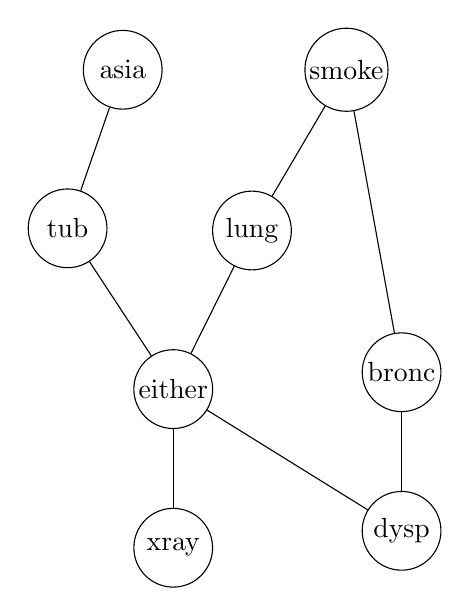
\begin{tikzpicture}[latent/.append style={minimum size=1cm},obs/.append style={minimum size=2cm}] %
    \node[latent] (asia) {asia} ; %
    \node[latent, right=of asia,xshift=0.8cm] (smoke) {smoke} ; %
    \node[latent, below=of asia,xshift=-0.7cm] (tub) {tub} ; %
    \node[latent, right=of tub, below=of smoke,xshift=-1.2cm] (lung) {lung};
    \node[latent, below=of lung,xshift=-1cm] (either) {either};
    \node[latent, below=of smoke,yshift=-1.8cm,xshift=0.7cm] (bronc) {bronc};
    \node[latent, below=of bronc] (dysp) {dysp};
    \node[latent, below=of either] (xray) {xray};
    \draw (asia)--(tub) ; %
    \draw (tub) -- (either);
    \draw (lung) -- (either);
    \draw (smoke)--(lung);
    \draw (smoke)--(bronc);
    \draw (bronc)--(dysp);
    \draw(either)--(dysp);
    \draw (either)--(xray);
  \end{tikzpicture}
\end{figure}
}
\only<5>{
Recall that $S_{tub,lung} = \emptyset$, which means we can introduce a v-structure $\textrm{tub} \rightarrow \textrm{either} \leftarrow \textrm{lung}$. We may also introduce the v-structure $\textrm{either} \rightarrow \textrm{dysp} \leftarrow \textrm{bronc}$.
\begin{figure}
  \centering
  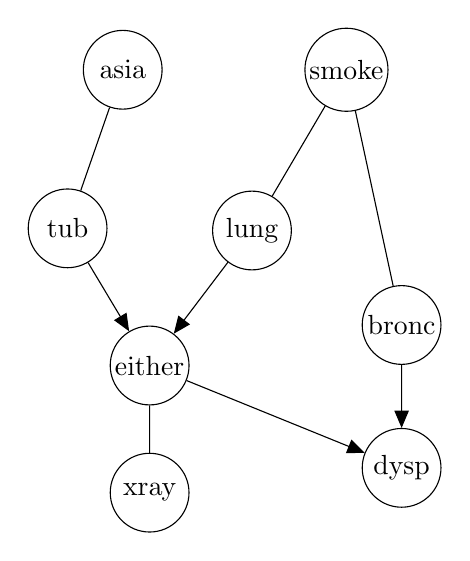
\begin{tikzpicture}[scale=0.6,latent/.append style={minimum size=1cm},obs/.append style={minimum size=2cm}] %
    \node[latent] (asia) {asia} ; %
    \node[latent, right=of asia,xshift=0.8cm] (smoke) {smoke} ; %
    \node[latent, below=of asia,xshift=-0.7cm] (tub) {tub} ; %
    \node[latent, right=of tub, below=of smoke,xshift=-1.2cm] (lung) {lung};
    \node[latent, below=of lung,xshift=-1.3cm,yshift=0.3cm] (either) {either};
    \node[latent, below=of smoke,yshift=-1.2cm,xshift=0.7cm] (bronc) {bronc};
    \node[latent, below=of bronc,yshift=0.2cm] (dysp) {dysp};
    \node[latent, below=of either,yshift=0.4cm] (xray) {xray};
    \draw (asia)--(tub) ; %
    \edge {tub}{either};
    \edge {lung}{either};
    \draw (smoke)--(lung);
    \draw (smoke)--(bronc);
    \edge {bronc}{dysp};
    \edge {either}{dysp};
    \draw (either)--(xray);
  \end{tikzpicture}
\end{figure}
}



\end{frame}


\section{Local PC Algorithm}

\subsection{Notation}
\begin{frame}
\frametitle{Notation}
\begin{itemize}
\item Let $X$ be a node in a DAG $\mathcal{G}$ (denoted as $X \in \mathcal{G}_V$). We denote the parent set of $X$ as $Z = pa(X)$
\item Our goal is to estimate the causal effect of $X$ on another node $Y$, i.e. $p(y \mid do(X=x))$, which can be calculated by
\begin{align*}
p(y \mid do(X=x)) &= \int_z p(y \mid do(x),z)p(z \mid do(x)) dz \\
&= \int_z p(y \mid x,z)p(z) dz \quad \textrm{Pearl (2000)}
\end{align*}
The last statement only requires conditional distributions that may be estimated from observational data.
\end{itemize}
\end{frame}

\begin{frame}
\frametitle{Notation}
\begin{itemize}
\item For a linear Structural Equation Model (SEM), the causal effect of $X$ on $Y$ is defined by
\begin{align*}
\frac{\partial}{\partial x} \mathbb{E}(Y \mid do(X=x)) &= \frac{\partial}{\partial x} \mathbb{E}(\beta x + \gamma^\top Z \mid do(X=x)) \\
&= \frac{\partial}{\partial x} \left\{ \beta x + \gamma^\top \mathbb{E}(Z) \right\}  \\
&= \beta
\end{align*}
where $(\beta,\gamma)$ is the regression coefficient of $Y$ on $(X,Z)$ (i.e. $\mathbb{E}(Y \mid X,Z) = \beta X + \gamma^\top Z$.
\item To estimate the causal effect, we only need to learn the parent set of $X$.
\end{itemize}

\end{frame}

\subsection{Motivation}

\begin{frame}
\frametitle{Motivation}
\begin{itemize}
\item Since we only need a node's parent set to estimate the causal effect, if we could estimate the local structure around a node, and use this result to estimate causal effects with reduced computational complexity
\item Nandy, Maathuis, and Richardson have found an algorithm to estimate causal effects with many \textit{potential} parent sets. It would improve the efficiency of their algorithm to minimize the amount of potential parent sets using a local structure learning algorithm. 
\end{itemize}
\end{frame}

\subsection{The Algorithm}

\begin{frame}{Idea}
In order to perform this estimation, we would need to be given the neighbors of $X$, denoted as $N$, where $N = N_1 \cup N_2$, and 
$$ N_1 = pa(X) \cup ch(X) \cup sp(X) $$
is the set of first-order neighbors, with 
\begin{itemize}
\item $ch(X) = \{x' \in \mathcal{G}_V: X \rightarrow x' \}$ 
\item $sp(X) = \{X' \in \mathcal{G}_V: ch(X) \cap ch(X') \neq \emptyset \}$
\item For a node $v \in \mathcal{G}_V$, let $N_1(v)$ denote the first-order neighbors of $v$
\end{itemize}
$N_2$ is the set of second-order neighbors, which we define as
$$ N_2 = \bigcup_{n \in N_1} N_1(n) $$
That is, $N_2$ is the union of the first-order neighbors for each of the first-order neighbors of the node of interest.
\end{frame}

\begin{frame}{Idea}
\begin{itemize}
\item Given the neighbors for our node of interest, we would proceed to use the PC algorithm to estimate the local structure. 
\item It may also be of interest to have a set of target nodes to consider. In this case, when proceeding through the PC Algorithm, we would \textit{not} have a complete graph on all the nodes being considered. Rather, we would only create complete graphs for each neighborhood.
\end{itemize}
\end{frame}


\subsection{Visualization}

\begin{frame}
\frametitle{Visualizing the Local PC Algorithm}
\only<1>{
Suppose the variable of interest is smoke.
\begin{figure}
  \centering
  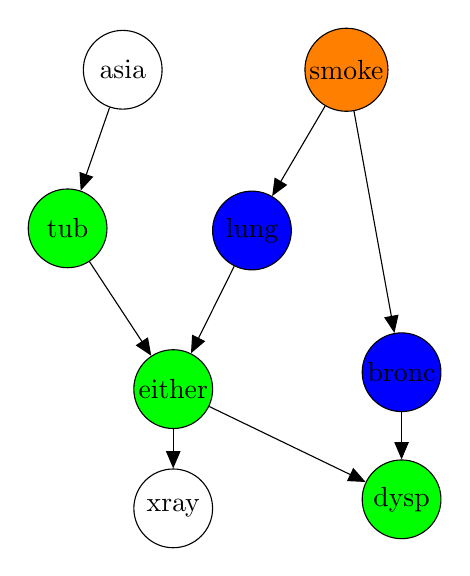
\begin{tikzpicture}[latent/.append style={minimum size=1cm},obs/.append style={minimum size=2cm}] %
    \node[latent] (asia) {asia} ; %
    \node[latent, right=of asia,xshift=0.8cm,fill=orange] (smoke) {smoke} ; %
    \node[latent, below=of asia,xshift=-0.7cm,fill=green] (tub) {tub} ; %
    \node[latent, right=of tub, below=of smoke,xshift=-1.2cm,fill=blue] (lung) {lung};
    \node[latent, below=of lung,xshift=-1cm,fill=green] (either) {either};
    \node[latent, below=of smoke,yshift=-1.8cm,xshift=0.7cm,fill=blue] (bronc) {bronc};
    \node[latent, below=of bronc,yshift=0.4cm,fill=green] (dysp) {dysp};
    \node[latent, below=of either,yshift=0.5cm] (xray) {xray};
    \edge {asia}{tub} ; %
    \edge {tub}{either};
    \edge{lung}{either};
    \edge{smoke}{lung};
    \edge{smoke}{bronc};
    \edge{bronc}{dysp};
    \edge{either}{dysp};
    \edge{either}{xray};
  \end{tikzpicture}
\end{figure}
}
\only<2>{
We start with a complete graph, only considering the neighborhood of smoke
\begin{figure}
  \centering
  \begin{tikzpicture}[latent/.append style={minimum size=1cm},obs/.append style={minimum size=2cm}] %
    \node[latent,xshift=0.8cm] (smoke) {smoke} ; %
    \node[latent, left=of lung,xshift=-0.7cm] (tub) {tub} ; %
    \node[latent, right=of tub, below=of smoke,xshift=1.5cm] (lung) {lung};
    \node[latent, below=of lung,xshift=-3cm] (either) {either};
    \node[latent, below=of smoke,yshift=-1.8cm,xshift=1.7cm] (bronc) {bronc};
    \node[latent, below=of bronc,xshift=-1.1cm,yshift=0.5cm] (dysp) {dysp};
    \draw (smoke)--(tub) ; %
    \draw (smoke)--(either);
    \draw (smoke)--(lung);
    \draw (smoke)--(dysp);
    \draw (smoke)--(bronc);
    \draw (tub)--(either);
    \draw (tub)--(lung);
    \draw (tub)--(dysp);
    \draw (tub)--(bronc);
    \draw (either)--(lung);
    \draw (either)--(dysp);
    \draw (either)--(bronc);
    \draw (lung)--(dysp);
    \draw (lung)--(bronc);
    \draw (dysp)--(bronc);
  \end{tikzpicture}
\end{figure}
}
\only<3>{
After completing the PC algorithm on this local set of nodes, we obtain
\begin{figure}
  \centering
  \begin{tikzpicture}[latent/.append style={minimum size=1cm},obs/.append style={minimum size=2cm}] %
    \node[latent,xshift=0.8cm] (smoke) {smoke} ; %
    \node[latent, left=of lung,xshift=-1.7cm] (tub) {tub} ; %
    \node[latent, right=of tub, below=of smoke,xshift=-0.5cm] (lung) {lung};
    \node[latent, below=of lung,xshift=-1cm] (either) {either};
    \node[latent, below=of smoke,yshift=-1.8cm,xshift=2.7cm] (bronc) {bronc};
    \node[latent, below=of bronc,xshift=-1.1cm,yshift=0.5cm] (dysp) {dysp};
    \draw (smoke)--(lung);
    \draw (smoke)--(bronc);
    \edge {lung} {either};
    \edge{tub}{either};
    \edge{either}{dysp};
    \edge{bronc}{dysp};
  \end{tikzpicture}
\end{figure}
}

\end{frame}

\section{Conclusion}

\begin{frame}
\frametitle{Future Research}
\begin{itemize}
\item Find an efficient way to estimate the neighborhood of a node
\item Compare the population version of the Local PC algorithm to that of the PC algorithm to see how accurate we are with only a few target nodes
\item Use generated data and compare the accuracy between the normal PC algorithm and the local algorithm. We expect to make some gains in this area because of fewer significance tests
\end{itemize}
\end{frame}

\begin{frame}
\frametitle{References}
\begin{enumerate}
\item Kalisch, M. and B\"uhlmann, P. (2007), ``Estimating high-dimensional directed acyclic graphs with the PC-algorithm," \textit{Journal of Machine Learning Research}.
\item Nandy, P., Maathuis, M. H., and Richardson T.S. (2017), ``Estimating the Effect of Joint Interventions From Observational Data in Sparse High-Dimensional Settings," \textit{Annals of Statistics}.
\end{enumerate}
\end{frame}

\begin{frame}
\frametitle{Questions}
\begin{center}
\Large Thank you
\end{center}
\end{frame}





\end{document}